\section{Frozen frontier judges on human ratings}
\label{sec:frozen}

% Provenance: experiments 21, 23, 26, 28 (frozen judges, calibration head); 02, 09, 10, 12, 14, 16, 18, 19, 20 (75 retrospective VeriBench artifacts).
Here the foundation model stays frozen and we calibrate only its reported category probabilities, so the comparison isolates the training objective from judge quality.
Each judge forecast $p$ passes through the 27-setting head of Equation~\eqref{eq:head}.
A CE fit and a Pearson fit choose among the same settings from the same training ratings (\appref{app:protocols}).
Experiment 28 has the widest coverage: five frontier judges (GPT-6 Astra, Claude Opus 5.5, Kimi K3, GLM 5.3, DeepSeek V4.1 Flash) on 2{,}350 label-free requests from five public rating sets.
Three come from ChaosNLI~\citep{nie2020chaosnli}, with 100 human labels per item: random subsets of the SNLI (600 items), MNLI-matched (600) and alphaNLI (400) parts.
Two are the chatbot-safety sets of DICES~\citep{aroyo2023dices}: DICES-350 (all 350 conversations, 123 ratings each) and DICES-990 (400 conversations, 69--76 ratings each).
We fixed the protocol and the request hashes before any judge call or label join.
Pearson and RPS inherit an ordinal coding that is an assumption: we read entailment as agreement and DICES as a harm scale (No $<$ Unsure $<$ Yes).
The SNLI and MNLI-matched parts keep only items whose original labels were not unanimous, so they over-represent disagreement.
AlphaNLI has two classes, so its mean fixes the distribution, and it serves as a control.
We test on held-out folds and score each held-out item against its entire empirical human distribution, with 200 training draws per fold and condition.
Budgets run from 4 to 256 ratings with one rating per item and from 10 to 320 ratings with five per item.

\begin{figure*}[t]
\centering
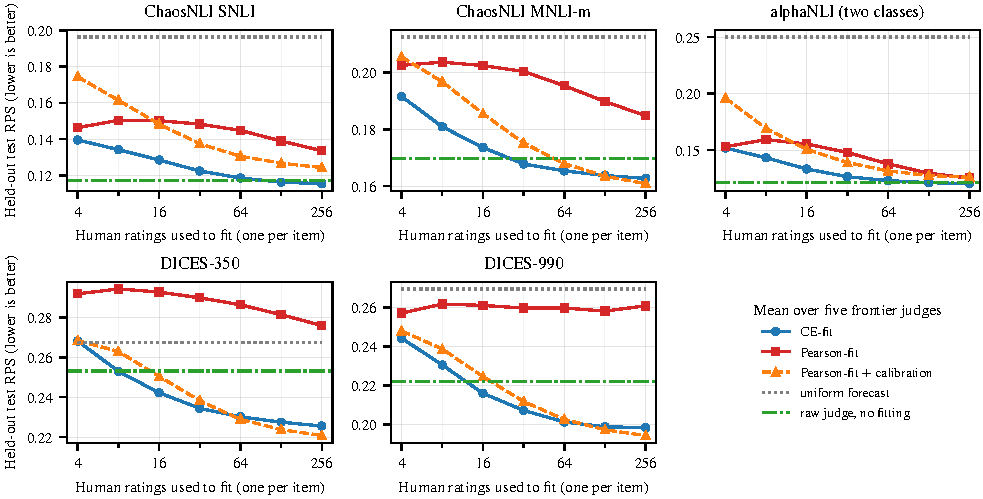
\includegraphics[width=\textwidth]{figures/fig_exp28.pdf}
\caption{\textbf{CE-fit passes the uniform forecast and Pearson-fit after a handful of ratings, but the unfitted judge is hard to beat on ChaosNLI, and a calibrated Pearson fit ends slightly lower on MNLI-matched and DICES.}
Learning curves of frozen judges with a calibration head on five public rating sets.
Vertical axis: held-out test ranked probability score (RPS), mean over the five frontier judges (0--1; lower is better); horizontal axis: number of human ratings spent on fitting, one rating per item.
Test data: held-out folds of ChaosNLI (SNLI, MNLI-matched, alphaNLI) and DICES (DICES-350 with 350 conversations, DICES-990 with a 400-conversation sample), each item scored against its full empirical human distribution; 200 training draws per fold.
Blue: CE-fit; red: Pearson-fit; orange dashed: Pearson-fit followed by distribution calibration on the same ratings; dotted gray: uniform forecast; dash-dotted green: the judge's raw forecast with no fitting.
Both fits search the same 27 calibration settings exhaustively (ties to the setting nearest the identity), so each is the exact optimum within that family.
No interval is drawn (see \Cref{tab:exp28}).}
\label{fig:exp28}
\end{figure*}

\paragraph{Result.}
CE-fit beats Pearson-fit and a uniform forecast on held-out RPS after 4 to 8 ratings with one rating per item, or after 10 to 20 ratings with five per item, in all 25 judge-by-dataset cells.
The simultaneous one-sided 97.5\% lower bounds of both differences stay above zero from the listed break-even budget $N^\ast$ to the largest tested (\Cref{tab:exp28}).
At the largest budget CE-fit has the lower mean RPS in all 50 judge-by-dataset-by-condition cells.
Across all 325 comparison cells, Pearson-fit has the lower mean RPS in 25 (three at four ratings with one per item and 22 at ten ratings with five per item, where four or two training items give a correlation very little to work with), significantly so in 19.
On DICES, where the Pearson-fit curve is flat, the gap is large: at 256 ratings the mean RPS is 0.226 for CE-fit against 0.276 for Pearson-fit on DICES-350 and 0.198 against 0.261 on DICES-990.

\begin{table*}[t]
\caption{\textbf{A handful of ratings suffices to beat both baselines, but at 256 ratings the calibrated Pearson fit equals or beats the cross-entropy (CE) fit on MNLI-matched and on both DICES sets.}
Held-out ranked probability score (RPS) at 256 human ratings (one per item) and break-even budgets, experiment 28.
Mean over five frontier judges; RPS in $[0,1]$, lower is better; bold marks the lowest value in the row.
Unif.: uniform forecast; Raw: the judge's own forecast with no fitting; Pearson-fit+cal.: a Pearson fit followed by train-only calibration of grade frequencies in four quantile bins of the expected score.
$N^\ast$: the smallest number of training ratings from which the simultaneous one-sided 97.5\% lower bounds of ``test RPS of the Pearson-fit judge minus test RPS of the CE-fit judge'' and ``test RPS of the uniform forecast minus test RPS of the CE-fit judge'' both stay above zero at every larger budget; ranges are across the five judges, with one (1/item) and five (5/item) ratings per item.
Test: held-out folds of each rating set, 200 training draws per fold; 4{,}000 bootstrap resamples of held-out items; both fits search the same 27 calibration settings exhaustively.}
\label{tab:exp28}
\centering\small
\begin{tabular}{lrrrrrcc}
\toprule
Rating set & Unif. & Raw & CE-fit & Pearson-fit & Pearson-fit+cal. & $N^\ast$ (1/item) & $N^\ast$ (5/item) \\
\midrule
ChaosNLI SNLI & 0.196 & 0.117 & \textbf{0.115} & 0.134 & 0.124 & 4 & 20 \\
ChaosNLI MNLI-m & 0.213 & 0.170 & \textbf{0.163} & 0.185 & 0.161 & 4 & 20 \\
alphaNLI (two classes) & 0.250 & 0.121 & \textbf{0.120} & 0.125 & 0.126 & 4--8 & 20 \\
DICES-350 & 0.267 & 0.253 & \textbf{0.226} & 0.276 & 0.221 & 8 & 10--20 \\
DICES-990 & 0.269 & 0.222 & \textbf{0.198} & 0.261 & 0.194 & 4 & 20 \\
\bottomrule
\end{tabular}

\end{table*}

\paragraph{CE is one way to fit the shape, not the only way.}
Against the unfitted judge the fitted head often loses: the raw forecast has significantly lower RPS than CE-fit in 156 of 325 cells (134 on ChaosNLI, where strong frontier judges already forecast the distribution well) and in 17 of 25 at eight ratings with one per item.
CE-fit has a sustained win over it (lower bound above zero at every larger budget) in 28 of 50 judge-by-set-by-condition cells: 2 of 10 on SNLI and on alphaNLI, 6 of 10 on MNLI-matched, 10 of 10 on DICES-350 and 8 of 10 on DICES-990.
A Pearson fit followed by calibration into grade frequencies, itself a proper-loss step, has lower mean RPS than CE-fit with one rating per item from 64 ratings on DICES-350 and from 128 on DICES-990 and MNLI-matched, by a few thousandths at 256 ratings (\Cref{tab:exp28}).
We read this as support for the argument, not a counterexample: what fails is selection or training by correlation \emph{alone}, and any step that fits the shape with a proper loss repairs it.

\paragraph{Other human ratings agree in direction and are mixed in size.}
\appref{app:extra} gives details and tables.
(1) On 160 student homework answers graded twice, CE-fit has lower held-out RPS than Pearson-fit for each of five frontier judges at every one of seven budgets (35 of 35 cells).
The preregistered descending test passes down to 8 ratings for two judges and fails at 256 for three (experiments 21 and 26).
For Qwen3.5-9B at 256 ratings the Pearson fit has the higher held-out correlation ($0.620$ against $0.556$) yet predicts a mean grade of $2.79$ for a human mean of $4.31$.
(2) On public benchmarks with a weaker judge (KonIQ-10k, SummEval, dialogue, MovieLens; experiment 23), direct CE selection beat direct Pearson selection at the largest budget on three of the four; on SummEval the Pearson fit won (RPS $0.144$ against $0.284$ at 768 ratings, the CE fit having selected the uniform forecast).
The margin over strong controls is small or absent in all four, and a calibrated Pearson score did at least as well as CE at the largest budget in all four.
(3) On the 75 retrospective theorem artifacts (195 expert ratings; Section~\ref{sec:limits} lists the experiments that reuse them), CE-trained mixtures and heads have lower test RPS than Pearson-trained ones in most pools and sizes, by $0.003$ to $0.090$ (experiments 10, 18 and 20).
At three training families CE ties on three pools and loses on the open-weight pool (experiment 20).
Choosing a single judge depends on the pool.
Selection by Pearson matched or beat selection by CE on the 44 historical scalar-vote judges, whereas selection by CE won on the 15 closed-weight judges with native probabilities, the 39 open-weight judges with three scalar votes and the combined 59 (experiment 20).
Pool format and model weights are confounded.
